\subsection{Smart Contract Workflow}

\todo{Clean up this section}

We wish to transfer assets from one blockchain to another and then back. When
assets can be transferred from one blockchain to another but not back, we call
it a \emph{one-way peg}. If assets can also be moved back, we call it a
\emph{two-way peg}. In each individual transfer of an asset, we have a
particular \emph{source blockchain}, from which the asset is moved, and a
particular \emph{target blockchain}, to which the asset is moved. In a sidechain
setting of two blockchains that are two-way pegged, both blockchains can
function as a source and a target blockchain for different transfers.

\begin{figure}[H]
    \vspace{-2em}
    \caption{Basic information transfer between two blockchains}
    \centering
    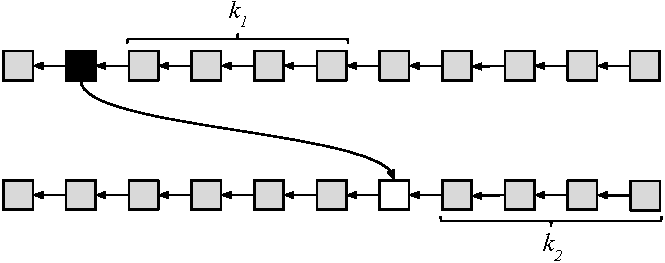
\includegraphics[width=0.7 \columnwidth,keepaspectratio]{chapters/sidechains/figures/events.pdf}
    \label{fig.events}
    \vspace{-2em}
\end{figure}

While the motivation for the construction is to be able to move assets from one
blockchain to another, we generalize the notion of sidechains from this strict
setting. In general, we would like the target blockchain to be able to react to
any \emph{event} that occurs on the source blockchain. Such events can be the
fact that a transaction with a particular \textsc{txid} took place, that a
certain account was paid a certain amount of money, or that a particular smart
contract was instantiated. Our sidechain construction allows the target
blockchain to react to events that took place on the source blockchain. This
reaction can be implemented in its target blockchain smart contracts. We
describe our construction in pseudocode similar to Ethereum' \emph{Solidity}. In
Solidity, \emph{events} can be fired arbitrarily from within a smart contract
and do not have a semantic interpretation. In this setting, events are defined
by Solidity using the \textsf{event} type and have an \emph{event name}, a
\emph{contract address} which fired them, as well as certain parameter values. A
contract can elect to fire an event with any name and any parameters of its
choice by invoking the \textsc{emit} command.

A high-level overview of cross-chain event transmission is shown in
Figure~\ref{fig.events}. The process is as follows. First, an event is fired in
the source blockchain, shown at the top. This could be any event that can be
emitted using Ethereum's \textsc{emit} command. This event firing is caused by a
certain transaction which is included at a certain block, indicated in black at
the top. This block is then buried under $k_1$ subsequent blocks within the
source blockchain, where the $k_1$ parameter is a security parameter of the
scheme depending on the specific parameters of the source
blockchain~\cite{backbone}. As soon as this confirmation occurs, the
target blockchain can react to the event, shown at the bottom. This reaction
occurs in a transaction which is included in a block within the target
blockchain, illustrated in white. As usual, the block needs to be confirmed by
waiting for $k_2$ blocks to be mined on top of it. It is possible that $k_1 \neq
k_2$ because of different blockchain parameters such as a difference in block
generation time or network synchrony.
In this figure, arrows between blocks of
the same blockchain indicate authenticated ancestry. The arrow between the two
blockchains indicates the data transfer needed for the event.

Using this basic functionality of event information exchange between
blockchains, we can construct two-way pegged sidechains. In such a construction,
an asset that exists on one blockchain will gain the ability to be \emph{moved}
to a different blockchain and back. We will use the example of moving ether, the
native asset of the Ethereum blockchain, from the Ethereum blockchain into the
Ethereum Classic blockchain and back. Such an action is different from
\emph{exchanging} ether (ETH), the native token of the Ethereum blockchain, with
ether classic (ETC), the native token of the Ethereum Classic blockchain.
Instead, the asset retains its nature; it maintains its price and its ability to
be used for the same purposes, while being governed by the rules of the new
blockchain, such as different performance, fees, features, or  security
guarantees. Furthermore, no counterparty or market is required to perform the
exchange; the transfer is something a party can do on its own.
